\section{Cryptography at work: PKI and TLS}
    \subsection{Recall of PKC}
    The Public Key Cryptography pros
    \begin{itemize}
        \item Private key is only known by the owner
        \item Confidentiality by encrypting with \textit{Receiver's Public Key}
        \item Non repudiation by encrypting with \textit{Sender's Private Key}
    \end{itemize}
    The cons are
    \begin{itemize}
        \item Low efficency: algorithms are 2-3 orders of magnitude slower than those for symmetric encryption
        \item How to distribute public keys
        \item There is still a big problem of Authentication: who ensures that the owner of a key pair is really the person whose real life name is "Alice".
    \end{itemize}  
    So in reality the \textbf{non repudiation} cannot be proven, cause we don't have the certified binding between an entity and it's public key. A mitigation for this is a \textbf{Digital signature}, a data item that vouches the origin and the integrity of a message, the originator of the message uses private key to sign the message, the recipient uses the public key of the sender to verify the origin. 
    
    \begin{figure}[h!]
        \centering
        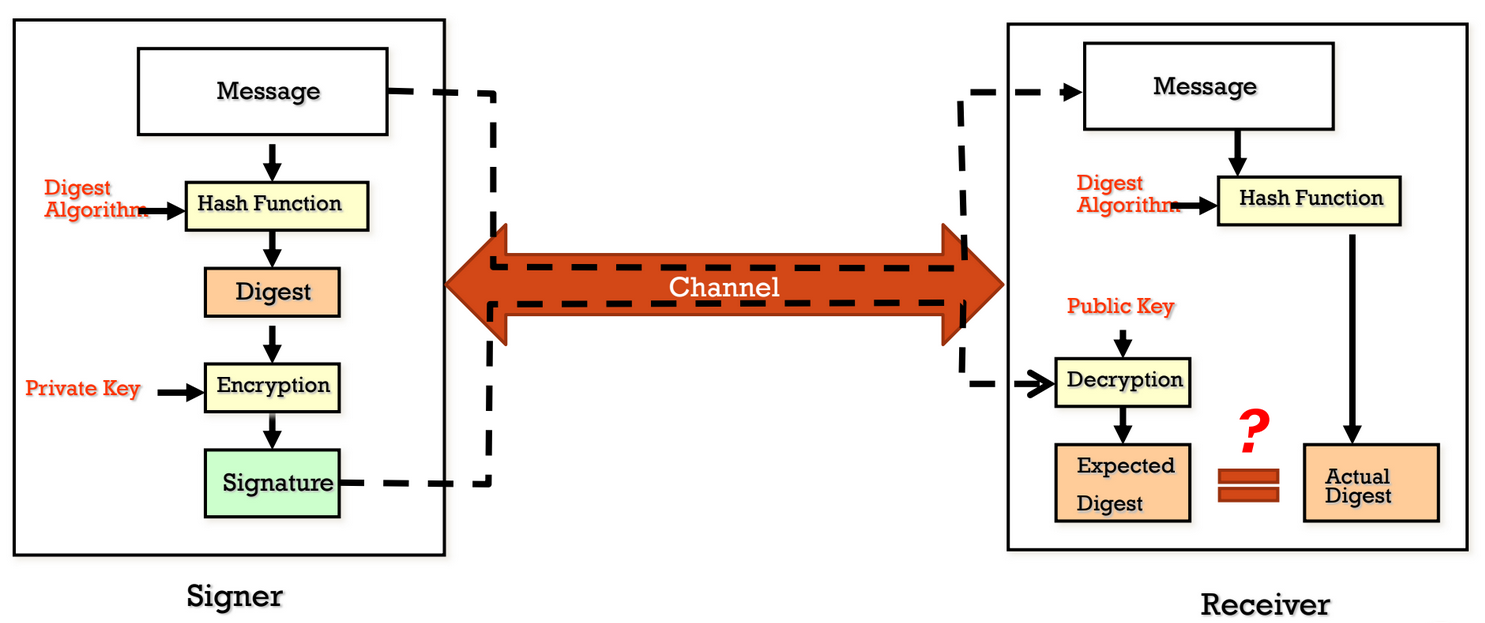
\includegraphics[scale=0.3]{images/PKCcomm.png}
    \end{figure}
    
    \FloatBarrier
    
    The problem now is who guarantees that the one using the key is entitled to do so?
    
    \subsection{Public Key Infrastructure (PKI)}
    The main requirement on public key is to be authentically bound to the identity of the party controlling the corresponding private key, another requirement is that parties relying on the correctness binding between public keys and corresponding party identities can be assured that the binding is still valid. Statisfying these two requirements is typically done by setting up a \textbf{Public Key Infrastructure}.
    
    \myparagraph{Digital Certificates}
    The initial proposal was to store the certificates fot binding public keys and identities as a bulletin boards so the public key and identities are listed. This is not scalable and has a single point of failure. Another propose was to hardcode the public key in the software, this approach was used in IoT at first but deprecated when discovered that this leads at possible vulnerability doing reverse engineering. 
    
    A widely adopted solution is the use of \textbf{digital certificates}, are digital objects containing data including the identity and the public key that are signed by a Trusted Third Party \textbf{(TTP)}, it bind an entity's Public Key and one or more attributes concerning its Identity (entity can be a person, an hardware component, a service ...). A Digital Certificate is issued and signed by a TTP that is also called Certificate Authority \textbf{(CA)}. The standard for certificates is the X.509, the validity of this certificate last for 6/12 month and at the end has the CA digital signature to prove the authenticity. For now this only moves the problem of checking the correctness of the binding between identity and public key to the distribution and keeping up to date the TTP's public key to check the authenticity of the certificate. This infinite regression problem is solved hardcoding the TTP public keys into the browsers.
    
    \subsection{Public Key Infrastructure}
    A Public Key Infrastructure \textbf{(PKI)} is an arrangement that binds public keys with respective identities of entities. The binding is established through a process of registration and issuance of certificates at and by a \textbf{CA} (Certificate Authority). The PKI role that assures valid and correct registration is called a \textbf{RA} Registration Authority. A third-party Validation Authority \textbf{(VA)} can provide an entity information on behalf the CA. Also has a Certificate distribution system that is composed of the repository for certificates and the CRL (Certificate Revocation List).
    
    So a PKI is a system that provides for a TTP to vouch for user identities and allows binding of public keys to subjects. Components:
    \begin{itemize}
        \item root Certificate Authority (CA), the most significant element in the CA hierarchy, root CA authorizes subordinate CAs. The subordinate CAs is responsable for issuing certificates.
        \item Registration Authority (RA) that verifies information in a certificate request, certificate are not issued until RA validation.
        \item Cryptographic Practices Statement (CPS) that is a declaration of the security that the organization is implementing.
        \item Certificate Revocation List (CRL) that tell us if the certificate is still valid or it has been revoked
    \end{itemize}
    
    \begin{figure}[h!]
        \centering
        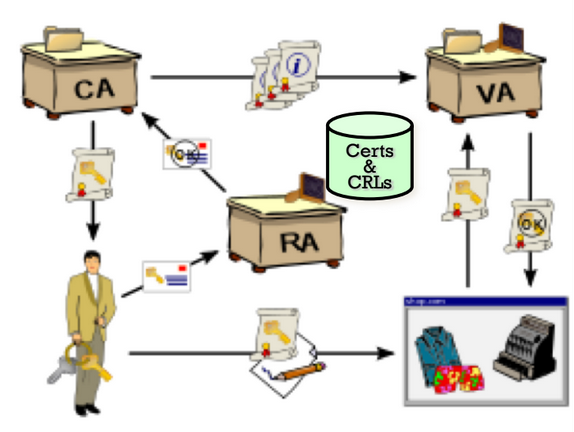
\includegraphics[scale=0.3]{images/PKI.png}
        \caption{The PKI infrastructure}
        \label{fig:pki}
    \end{figure}
    
    \FloatBarrier
    
    To obtain a certificate a user generates a Public and Private key-pair or is assigned a key-pair by some authority in their organization, user request the certificate of the CA server. The CA responds with its Certificate including its Public Key and its Digital Signature signed using its Private Key. User gathers all information required by the CA Server to obtain its certificate, it also sends a certificate request to the CA consisting of her Public Key and additional information. The certificate request is signed by user Private Key. CA gets the certificate request, verifies user identity and generates a certificate for user, binding her identity and her Public Key. The signature of CA verifies the authenticity of the Certificate. CA issues the certificate to user.
    \begin{figure}[h!]
        \centering
        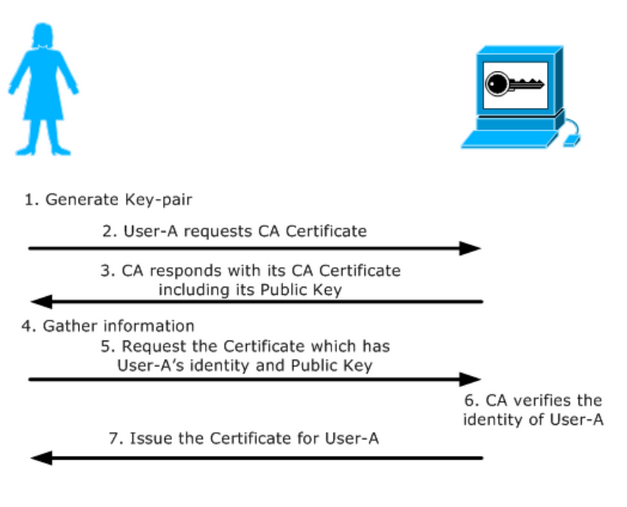
\includegraphics[scale=0.3]{images/obtaincertificate.png}
        \caption{How to obtain a certificate}
        \label{fig:obtainingc}
    \end{figure}
    
    \FloatBarrier
    
    Let's focus on the procedure of requesting, is also called the step in which a Certificate Signing Request \textbf{(CSR)} is generated, it contains information identifying the requester, the public key chosen by the requester, additional proofs of identity and a digital signature.

    TTPs must be trustworthy in issuing certificates only to the right parties, in the past TTPs were involved in incidents resulting in certificates issued to the "wrong" parties. As a result google and other companies launched an initiative for building a platform for checking certificate transparency.

    Another thing is that we need to know if certificates are still valid or not, this is done locally with the CRL but it has to always be up-to-date, or using online certificate status protocol (OCSP) that provides an API to check if a certificate is in the CRL but it requires high bandwidth.
    
    \subsection{SSL and TLS}
    \subsubsection{Introduction}
    Secure Sockets Layer \textbf{(SSL)} and Transport Layer Security \textbf{(TLS)} wants to provide user with identity of page origin and indicate to user that page contents were not viewed or modified by a network attacker. HTTPS that stays for HTTP over TLS/SSL provides authentication of the website and associated web server with which one is communicating (protection against MITM), bidirectional encryption of communications between a client and a server.
    \subsubsection{TLS overview}
    TLS is used in client-server applicatin, it consists of two main protocols: the \textbf{Handshake protocol} that uses PKC to establish a shared secret key between the client and the server and the \textbf{Record protocol} that uses the key established in the handshake to protect communication between the client and the server.
    \myparagraph{Handshake protocol}
    Two parties: client and server, they negotiate the version of the protocol and the set of cryptographic algorithms to be used, it authenticate client and server and use public key to establish a shared secret
    \myparagraph{Record protocol}
    It provides confidentiality and Integrity, on the send side it fragment data into blocks applying authentication and encryption primitives to each block, finally handing the block to TCP for transmission over the network. On the receice side the blocks are decrypted and verified for message integrity, then reassembled and delivered to the higher level protocol.
    \subsubsection{TLS 1.2: Details of the handshake}
    
    \begin{figure}[h!]
        \centering
        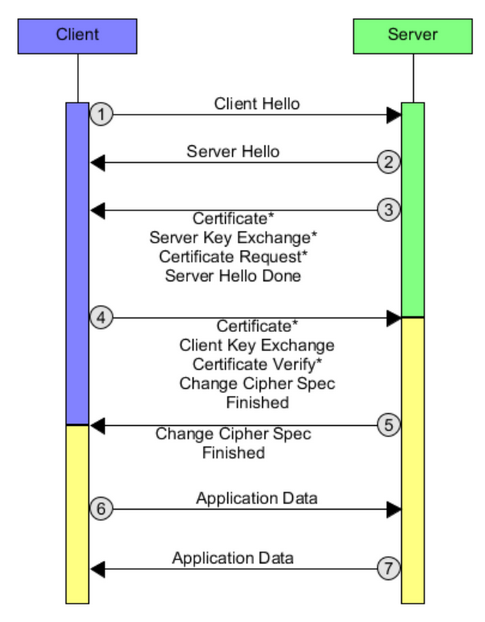
\includegraphics[scale=0.4]{images/handshakeTls.png}
        \caption{TLS handshake}
        \label{fig:tlsH}
    \end{figure}
    
    \FloatBarrier
    
    \myparagraph{Step 1}
    At the first step the client send the Client \textbf{Hello} Message that contains the version of the protocol that the client wants to use and a list of supported cipher suite. A cipher suite is a set of algorithms that help secure a network connection that uses TLS/SSL, usually it includes a key exchange algorithm, a bulk encryption algorithm and a message authentication code (MAC) algorithm. It can also include signatures and authentication algorithms
    \myparagraph{Step 2}
    The server send the server \textbf{Hello} message that contains the chosen protocol, the chosen cipher suite and the session ID
    \myparagraph{Step 3}
    If the client requested an authenticated connection, the server must send a X.509 certificate, a server can request the client to be authenticated too. \textbf{Client Key Exchange}: message sets the premaster secret that will be later used to generate the Master Secret.
    \myparagraph{Step 4}
    If the client has received a Certificate Request message, it must send a X.509 certificate. \textbf{Client Key Exchange}: message sets the pre-master secret that will be later used to generate the master secret. There is also the Certificate Verify, a message that provides explicit verification on the client certificate.

    A pre-master secret is the value obtained from the key exchange, in DH the pre-master secret is $g^{ab} mod p$. The master secret is derived from it by using a pseudo random function (PRF), from the master secret both client and server derive multiple session keys by using again PRF.
    \myparagraph{Step 5}
    Send the Change Cipher Spec, message sent by both parties, once received the partecipant transitions to the agreed cipher suite. Finished message is generate by hashing the entire handshake and sent by both parties
    \myparagraph{Step 6-7}
    From now every message sent will be encrypted using the shared key.
    \\\\
    How SSL and TLS provide identification, authentication, confidentiality and integrity? For the \textbf{server authentication} the client uses the server's public key to encrypt the data that is used to compute the secret key, the server can generate the secret key only if it can decrypt that data with the correct private key. For \textbf{client authentication} the server uses the public key in the client certificate to decrypt the data the client sends during step 4 of the handshake. The exchange of secret messages confirm that the authentication is complete. If any of the authentication steps fail, the handshake fails and the session terminates. The exchange of digital certificates during the SSL or TLS handshake is part of the authentication process.
    
    The \textbf{confidentiality} is provided by a combination of symmetric and asymmetric encryption to ensure message privacy, the encryption algorithms are agreed during the handshake. There is no key distribution problem because TLS use asymmetric encryption.
    
    The \textbf{integrity} is provided by using a Message Authentication Code \textbf{(MAC)}, the use of TLS does ensure data integrity, provided that the CipherSpec in the channel definition uses a suitable hash or MAC algorithm. The MAC is a tag used to confirm that the message came from the stated sender and the MAC allows verifiers to detect any changes to the message content. A MAC algorithm is a family of cryptographic functions that can be used to provide data origin authentication as well as data integrity by producing a MAC on arbitrary messages.
    
    \subsubsection{TLS Vulnerabilities}
    TLS soffers from some security issues for a few reasons:
    \begin{itemize}
        \item Backward compatibility: the protocol still supports weak cipher suites and broken hash functions.
        \item Logical flow: set of logical loopholes can be used to "trick" both client and server.
        \item Implementation issues: Libraries (like \textbf{Openssl}) contains bugs and some of them can be exploited to mount attacks.
    \end{itemize}   
    
    \myparagraph{Nonces}
    A nonce is an arbitrary number that can be used just once in a cryptographic communication, typically it is a pseudo random number issued by one of the parties in a protocol to ensure that old communications cannot be reused in replay attack

    \myparagraph{POODLE}
    The clien initiates the handshake and sends a list of supported SSL/TLS version, an attacker intercepts the traffic, performing a MITM attack and impersonates the server until the client agrees to downgrade the connection to SSL 3.0. At this point the attacker can exploit a weakness in one of the block ciphers supported by SSL 3.0 to guess cookies and other sensitive information.

    \myparagraph{HEARTBLEED}
    Found in the heartbeat extension of the popular OpenSSL library used to keep a connection alive as long as both parties are still there. If the client sent false data length, the server would respond with the data received by the client and random data from its memory to meet the length requirements specified by the sender. Sometimes this random data could be password, credit card number ecc...
    
    \subsection{TLS 1.3}
    It cleaned up the old TLS removing unsafe or unusued features, improved security with respect to modern techniques. It mantained the backward compatibility and encrypted more of the protocol. It has also a \textbf{faster handshake} with 0-RTT and 1-RTT handshake: RSA has been removed, and improved DH to send the required cryptographic parameters for key generation already included in its "hello". If we reuse a key we are in the 0-RTT case, this as an impact in terms of security because the more a key is used the higher is the risk.
    Removed support to algorithms that are a family of algorithm that have a feature of specific key agreement protocols that gives assurances that session keys will not be compromised even if long-term secrets used in the session key exchange are compromised. Now the cipher suites supported are 5 instead of the 319 in TLS 1.2 Added support to \textbf{forward secrecy}, it protects past session against future compromises of keys or password. For example if a long term secret in the session key exchange is compromised, the session will not be compromised. By generating a unique session key for every session a user initiates, the compromise of a single session key will not affect any data other than that exchanged.
    \textbf{Ephemeral Diffie-Hellman} differs from the standard DH in the way that static DH key exchanges always use the same DH private keys, DHE provide a temporary DH key every connection that is always different, this do not more provide the authentication so DHE has to be combined with an additional authentication mechanism.
    